
% !TEX encoding = UTF-8 Unicode

% This LaTeX was auto-generated from MATLAB code.
% To make changes, update the MATLAB code and republish this document.

\documentclass[12pt,final,twoside,notitlepage]{article}

% Encodage caractère et fonte
%\usepackage[utf8]{inputenc}
%\usepackage[T1]{fontenc}

% Langue: français	
\usepackage[spanish]{babel}
\usepackage{xspace}
\usepackage{fancyhdr}
\usepackage{amsmath}
\usepackage[left=3cm,right=3cm,top=2cm,bottom=6cm]{geometry}

% Utilisation de \nombre
\usepackage[autolanguage]{numprint} 

\usepackage{graphicx}
\usepackage{xcolor}
\usepackage{listings}
\definecolor{vertmatlab}{RGB}{28,160,55}
\definecolor{mauvematlab}{RGB}{155,71,239}
\definecolor{fond}{RGB}{246,246,246}
\definecolor{lightgray}{gray}{0.5}

\setlength{\parindent}{0pt}

\begin{document}
\lstset{
	language=Matlab,%
	inputencoding=utf8,%x-iso-8859-15,%
	extendedchars=true,%
	basicstyle=\footnotesize\ttfamily, % Standardschrift
	numberstyle=\tiny\color{gray},
	keywordstyle=\color{blue},
	commentstyle=\color{vertmatlab},
	stringstyle=\color{mauvematlab}\ttfamily,
	numbers=left,               % Ort der Zeilennummern
	numberstyle=\tiny\color{gray}, % Stil der Zeilennummern
	%	stepnumber=2,               % Abstand zwischen den Zeilennummern
	numbersep=5pt,              % Abstand der Nummern zum Text
	tabsize=2,                  % Groesse von Tabs
	breaklines=true,            % Zeilen werden Umgebrochen
	frame=tb,         
	%	keywordstyle=[1]\textbf,    % Stil der Keywords
	%	keywordstyle=[2]\textbf,    %
	%	keywordstyle=[3]\textbf,    %
	%	keywordstyle=[4]\textbf,   \sqrt{\sqrt{}} %
	showspaces=false,           % Leerzeichen anzeigen ?
	showtabs=false,             % Tabs anzeigen ?
	xleftmargin=17pt,
	framexleftmargin=17pt,
	framexrightmargin=0pt,
	framexbottommargin=4pt,
	backgroundcolor=\color{fond},
	showstringspaces=false,     % Leerzeichen in Strings anzeigen ?        
	literate={é}{{\'e}}1 {è}{{\`e}}1, % Accentuation française
}

\thispagestyle{fancy}
\lhead{\includegraphics[width=1.5cm]{ucr.png}}
\chead{\textbf{UNIVERSIDAD DE COSTA RICA\\FACULTAD DE CIENCIAS\\ESCUELA DE MATEMÁTICA}}
\rhead{
\includegraphics[width=4cm]{EMat.png}}

\textbf{\begin{center}
MA-0501 Análisis Numérico I\\ TAREA 1\\
\end{center}}


    
    
\section*{}




\begin{verbatim}publish('T1_Murillo','format','latex','stylesheet','matlab2latex.tex')\end{verbatim}

\begin{par}
	\textbf{Respuesta Corta}
\end{par}
\\
\begin{par}
	1) Para aproximar numéricamente la solución de la ecuación $|x^2-1|=0$ se puede usar el método de aproximaciones sucesivas pues se puede encontrar un conjunto convexo, compacto y no vacío en R que contenga las raíces y como la función es continua, entonces existe el punto fijo por el teorema 2.5. Además, el método de bisección no es factible usarlo pues la función no tiene imagánes negativas, el de Newton tampoco pues la derivada se indefine en dos puntos, igual que con el de secante.
\end{par}
\\
\begin{par}
	2) Al usar el método de Newton en la ecuación $x^{100} = 0$ se espera que este falle, pues $\frac{d(x^{100})}{dx} = 100x^{99}$, es importante notar que conforme se efectúe el proceso, como la raíz de esa ecuación es cero, la derivada se va a acercar a cero, por lo que se indefiniría.
\end{par}
\\
\begin{par}
	3) Para determinar numéricamente la multiplicidad de dicho cero, basta con calcular la derivada de f, después la de f´ y así sucesivamente, la multiplicidad estara dada por la cantidad de derivadas que hemos realizado hasta que se anule al evaluar c, i.e. la primera vez que se anule una de las derivadas al evaluar en c.
\end{par}
\\
\begin{par}
	4) No tiene sentido realizar mas de 52 iteraciones pues note que si realizamos 52 iteraciones el error estara dado por:
\end{par}

\begin{par}
	
\begin{align*}
e_{52} < \frac{1}{2^{53}}\abs(2-1) \\
\Rightarrow e_{52} < \frac{1}{2^{53}}
\end{align*}

\end{par}

\begin{par}
	el cual es menor que el epsilon de la maquina en precision doble.
\end{par}
\\
\begin{par}
	5a) Para el polinomio $p(x) = a_nx^n + ... + a_1x + a_0$, si se desea conocer $p(x_0)$ es necesario efectuar $(n^2+n)/2$ y n sumas.
\end{par}
\\
\begin{par}
	5b) Para este algoritmo, se deben realizar en cada iteración una suma y una multiplicación, como son n iteraciones, en total se realizan n sumas y n multiplicaciones.
\end{par}
\\
\begin{par}
	6) El polinomio de Lagrange para $f(x) = x^2 + 3x +1$ es él mismo, pues es un polinomio, de igual forma si se calcula obtenemos:
\end{par}

\begin{par}
	
\begin{align*}
\frac{(x-1)}{-1} \frac{(x-2)}{-2}+ 5 \left(\frac{x}{1} \frac{(x-2)}{1-2}\right) + 15 \left(\frac{x}{2} \frac{(x-1)}{2-1}\right) = x^2 + 3x +1
\end{align*}

\end{par}

\begin{par}
	\textbf{Desarrollo}
\end{par}

\begin{par}
	1) Al ejecutar el código suministrado, se obtiene para $n=10$ (note que en este caso se ejecuta el código)
\end{par}

\begin{lstlisting}
n = 1478;
f = []; g = [];
f(1)=0;
f(2)=1;
for i=2:(n-1)
    f(i+1)=f(i)+f(i-1);
end

g(n)=f(n);
g(n-1)=f(n-1);
for i=(n-1):-1:2
    g(i-1)=g(i+1)-g(i);
end
\end{lstlisting}

\begin{par}
	Sabemos que el término n de la sucesión de Fibonacci está dado por:
\end{par}

\begin{par}
	
\begin{align*}
f(n) = \frac{1}{\sqrt{5}} \left( \phi^n - \frac{(-1)^n}{\phi^n} \right)
\end{align*}

\end{par}

\begin{par}
	
tq \phi = \frac{1+ \sqrt{5}}{2}

\end{par}

\begin{par}
	Note que para n suficientemente grande la siguiente expresión tiende a 0
\end{par}

\begin{par}
	
\begin{align*}
\frac{(-1)^n}{\phi^n}
\end{align*}

\end{par}

\begin{par}
	Entonces, basta con resolver la siguiente desigualdad para $n$, pues en precisión doble el último valor que puede almacenar en la computadora es $2^{1023}$.
\end{par}

\begin{par}
	
\begin{align*}
 2^{1023} < \frac{\phi^n}{\sqrt{5}}
\end{align*}

\end{par}

\begin{par}
	Al calcular la expresión anterior se obtiene que $n > 1475,22$, i.e. n debe ser aproximadamente 1476.
\end{par}
\\
\begin{par}
	1b) Para números medianos f(1) y g(1) serán diferentes debido al redondeo pues la computadora únicamente puede guardar números completos si son menores de 10\^{}16, es por ello que para encontrar el mínimo valor de n donde f(1) y g(1) son diferentes basta con calcular:
\end{par}

\begin{par}
	
\begin{align*}
 10^{16} < \frac{\phi^n}{\sqrt{5}}
\end{align*}

\end{par}

\begin{par}
	Al calcular la expresión anterior se obtiene que $n > 78,23$, i.e. n debe ser aproximadamente 79. Es importante notar que igual al ejercicio anterior despreciamos la expresión que tiende a 0.
\end{par}
\\
\begin{par}
	1c)
\end{par}

\begin{lstlisting}
%Estimacion del inciso (a)

f(1476)
\end{lstlisting}

\begin{lstlisting}

ans =

  8.0776e+307


\end{lstlisting}
    
\begin{par}
	Note que en el inciso (a) obtuvimos que el mínimo valor en el que el algoritmo comienza a fallar es en 1476, sin embargo, esto no sucede así.
\end{par}

\begin{lstlisting}
f(1478)
\end{lstlisting}

\begin{lstlisting}

ans =

   Inf


\end{lstlisting}
    
\begin{par}
	No obstante, el algoritmo comienza a fallar tan solo 2 números después, en 1478.
\end{par}

\begin{lstlisting}
%Estimacion del inciso (b)

n = 79;
f = []; g = [];
f(1)=0;
f(2)=1;
for i=2:(n-1)
    f(i+1)=f(i)+f(i-1);
end

g(n)=f(n);
g(n-1)=f(n-1);
for i=(n-1):-1:2
    g(i-1)=g(i+1)-g(i);
end

f(1)
g(1)
\end{lstlisting}

\begin{lstlisting}

ans =

     0


ans =

     0


\end{lstlisting}
    
\begin{par}
	Observe que ambos valores siguen siendo el mismo
\end{par}

\begin{lstlisting}
n = 80;
f = []; g = [];
f(1)=0;
f(2)=1;
for i=2:(n-1)
    f(i+1)=f(i)+f(i-1);
end

g(n)=f(n);
g(n-1)=f(n-1);
for i=(n-1):-1:2
    g(i-1)=g(i+1)-g(i);
end

f(1)
g(1)
\end{lstlisting}

\begin{lstlisting}

ans =

     0


ans =

   8.9444e+15


\end{lstlisting}
    
\begin{par}
	Note que en este caso g(1) y f(1) son distintos, tan solo un numero mayor a lo calculado en el inciso (b)
\end{par}
\\
\begin{par}
	2a) Como la computadora no tiene implementada la división, entonces debemos intentar encontrar otra forma de usar Newton.
\end{par}

\begin{par}
	Note que: $f'(x) = \frac{-1}{x^2}$, entonces podemos escribir Newton como:
\end{par}

\begin{par}
	
\begin{align*}
c_k = c_{k-1} - x^2\left(\frac{1}{x} -b\right)
\end{align*}

\end{par}

\begin{par}
	Al simplificar obtenemos:
\end{par}

\begin{par}
	
\begin{align*}
 c_k = c_{k-1} + c_{k-1}(1-bc_{k-1})
\end{align*}

\end{par}

\begin{par}
	Para verificar las condiciones, suponga que $\displaystyle\lim_{n \to \infty} x_{n-1} = x$
\end{par}

\begin{par}
	Note que
\end{par}

\begin{par}
	
\begin{align*}
\lim_{n \to \infty} x_n = \displaystyle\lim_{n \to \infty} x_{n-1} + x_{n-1} - bx_{n-1}^2
\end{align*}

\end{par}

\begin{par}
	Entonces
\end{par}

\begin{par}
	
\begin{align*}
x = x + x -bx^2
\Rightarrow x = \frac{1}{b}
\end{align*}

\end{par}

\begin{par}
	
Como la función es de clase $C^2$, $f(1/b) = 0$ y $f'(1/b) \neq 0$, por el
teorema 2.1 podemos asegurar que existe un intervalo donde converge.

\end{par}
\\
\begin{par}
	2b) Implementamos el algoritmo anterior:
\end{par}
\begin{verbatim}function c1 = myDivision(c0, b)
c1 = c0 + c0*(1 -b*c0);
while(abs(c1-c0)\ensuremath{>}=eps)
c0 = c1;
c1 = c0 + c0*(1 -b*c0);\end{verbatim}
\begin{verbatim}end
end\end{verbatim}

\begin{par}
	2c)
\end{par}

\begin{lstlisting}
b = pi;
c0= linspace(0,1,1e5); %valores que toman los c0

c1 = myDivision(c0, b);

%Valor de convergencia en funcion de c0

xx = c0;
yy = nan(size(xx));

for i = 1: numel(xx)
    yy(i) = myDivision(xx(i), b);
end

figure
semilogx(xx,yy, 'MarkerSize', 20)

%Titulo
title('Gráfico 1 :Convergencia en función de c0')

%Nombrar ejes
xlabel('$x_0$ : valores iniciales', 'Interpreter', 'latex')
ylabel('Valores de convergencia', 'Interpreter', 'latex')
\end{lstlisting}

\begin{figure}[h!]
\centering
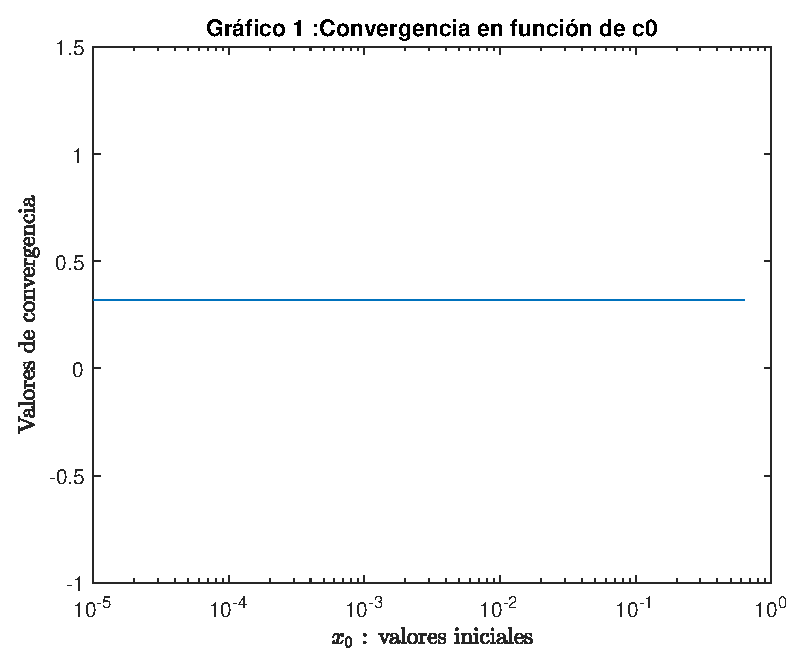
\includegraphics [width=4in]{T1_Murillo_01.eps}
\end{figure}

\begin{par}
	Tome delta de la siguiente forma:
\end{par}

\begin{par}
	
\begin{align*}
\delta = \frac{1}{5}
\end{align*}

\end{par}

\begin{par}
	
Entonces, tome $I = [\frac{1}{\pi} - \frac{1}{5}, \frac{1}{\pi} +
\frac{1}{5} ]$

\end{par}

\begin{par}
	
\begin{align*}
A = \max_{(x,y) \in I} |\frac{f''(x)}{f(y)}| &=  |\frac{2}{x^3y^2}|
\end{align*}

\end{par}

\begin{par}
	
Tome $\eta =\min(1, \frac{1}{A})$ , entonces podemos asegurar
convergencia por el teorema 2.21 en $[\frac{1}{\pi} - \eta, \frac{1}{\pi}
+ \eta]$, lo cual coincide con lo graficado.

\end{par}
\\
\begin{par}
	2d) Aplicaría bisección primero, para poder encontrar un x0 lo suficientemente cerca de su raíz.
\end{par}
\\
\begin{par}
	3a) Note que por conmutatividad del producto se sigue que
\end{par}

\begin{par}
	
\begin{align}
\prod_{i=1}^{N_c} f(y_i, \theta) &= \prod_{i}^{N_c} \binom{n_i}{y_i} \prod_{i}^{N_c} \theta^{y_i} \prod_{i}^{N_c} (1- \theta)^{n_i - y_i} \\
&\prod_{i}^{N_c} \binom{n_i}{y_i} \theta^{H} (1 - \theta)^{M}
\end{align}
\text{donde } $H = \displaystyle\sum_{i}^{N_c} y_i $ \text{y } $M = \displaystyle\sum_{i}^{N_c} n_i - y_i $.

\end{par}

\begin{par}
	Procedemos a calcular $l'(\theta)$ Note que
\end{par}

\begin{par}
	
\begin{align*}
 l(\theta) = \log(L(y_1, ... , y_N, \theta) = \log\left(\prod_{i=1}^{N_c} f(y_i, \theta)\right)
\end{align*}

\end{par}

\begin{par}
	Por (1) y (2), se sigue que
\end{par}

\begin{par}
	
\begin{align*}
   \log(L(y_1, ... , y_N, \theta) &= \log \left( \prod_{i}^{N_c} \binom{n_i}{y_i} \theta^{H} (1 - \theta)^{M} \right) \\
   &= \log\left(\prod_{i}^{N_c} \binom{n_i}{y_i}\right) + H \log(\theta) + M\log( 1-\theta)
\end{align*}

\end{par}

\begin{par}
	Entonces
\end{par}

\begin{par}
	
\begin{align*}
   l'(\theta) = \frac{H}{\theta} - \frac{M}{1- \theta}
\end{align*}

\end{par}

\begin{par}
	Al despejar e igualar a 0, obtenemos los puntos críticos de $l(\theta)$
\end{par}

\begin{par}
	
\begin{align*}
    l'(\theta) &= \frac{H}{\theta} - \frac{M}{1- \theta} = 0 \\
    &\Rightarrow \theta = \frac{H}{N}
\end{align*}

\end{par}

\begin{par}
	donde N = H+ M.
\end{par}

\begin{par}
	Además, este punto crítico en efecto es el máximo pues $l''(\theta) < 0$ y por el criterio de la segunda derivada podemos asegurar que es el máximo.
\end{par}
\\
\begin{par}
	3b)
\end{par}

\begin{lstlisting}
%Leemos el archivo
T = readtable('data.txt');
\end{lstlisting}
\\
\begin{par}
	3c)
\end{par}

\begin{lstlisting}
%Vectorizamos los datos
m = T.Machos;
h = T.Hembras;

%Procedemos a calcular el valor que maximiza los datos suministrados

%Cantidad total de machos
suma_m = sum(m);

%Cantidad total de hembras
suma_h = sum(h);

%Valor que maximiza
maximo = suma_h/(suma_m + suma_h)
\end{lstlisting}

\begin{lstlisting}

maximo =

    0.4946


\end{lstlisting}
\\   
\begin{par}
	3d)
\end{par}

\begin{lstlisting}
f = @(x) suma_h/x - suma_m/(1-x);

Secante(f,0.30,0.60)
\end{lstlisting}

\begin{lstlisting}

ans =

    0.4946


\end{lstlisting}
\\  
\begin{par}
	3e)
\end{par}

\begin{lstlisting}
[x,fval,exitflag,output,jacob] = fsolve(f,0.50);

% Resultado del fsolve
disp(x)

%Algoritmo usado
disp(output)
\end{lstlisting}

\begin{lstlisting}

Equation solved.

fsolve completed because the vector of function values is near zero
as measured by the value of the function tolerance, and
the problem appears regular as measured by the gradient.

    0.4946

       iterations: 1
        funcCount: 4
        algorithm: 'trust-region-dogleg'
    firstorderopt: 3.3382e-10
          message: 'Equation solved.↵↵fsolve completed because the vector of function values is near zero↵as measured by the value of the function tolerance, and↵the problem appears regular as measured by the gradient.↵↵<stopping criteria details>↵↵Equation solved. The sum of squared function values, r = 1.292470e-26, is less than↵sqrt(options.FunctionTolerance) = 1.000000e-03. The relative norm of the gradient of r,↵3.338242e-10, is less than options.OptimalityTolerance = 1.000000e-06.'


\end{lstlisting}
\\  
\begin{par}
	4a) Por el teorema 2.10 de las notas sabemos que basta con demostrar que una función es continua y que el valor absoluto de su derivada se puede acotar por una constante menor que 1 para que el proceso de iteración simple converja a su punto fijo. Note que $g(x) = x -(x^2 -3)/2$ es claramente continuo pues es un polinomio. Procedemos a analizar la derivada de g Note que $|g'(x) |= |1 -x|$, la cual es una función creciente y alcanza su máximo en su extremo derecho en el valor de 1, entonces podemos asegurar que para todo $x \in (a,b)$ sucede que $|g'(x)| < 1$.
\end{par}
\\
\begin{par}
	4b)
\end{par}

\begin{lstlisting}
g = @(x) x -(x.^2 -3)./2;
raiz = 1.732050807568877; %Valor de sqrt{3} con 15 decimales

[c, secS] = iterSimple(g, 1.5);


semilogy(1:numel(secS),abs(secS-raiz)/abs(raiz),'.-','MarkerSize',10);


%Titulo
title('Gráfico 2 :Error relativo en función del número de iteraciones')

%Nombrar ejes
xlabel('Cantidad de iteraciones')
ylabel('Error relativo')
\end{lstlisting}

\begin{figure}[h!]
\centering
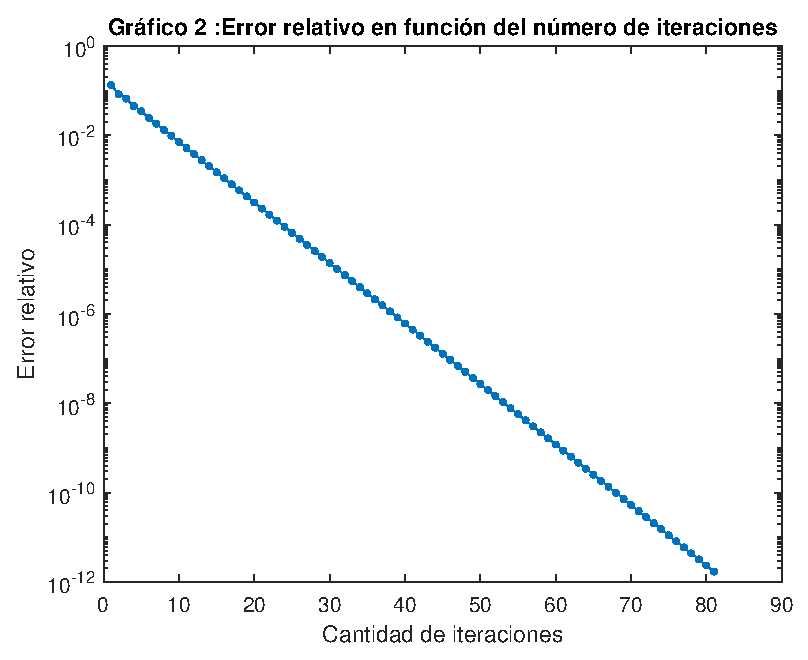
\includegraphics [width=4in]{T1_Murillo_02.eps}
\end{figure}
\\
\begin{par}
	¿Cual es la pendiente de la recta en su grafica? ¿Qué representa dicha pendiente?
\end{par}

\begin{par}
	Procedemos a calcular la pendiente de la recta
\end{par}

\begin{lstlisting}
pendiente = ((abs(secS(36)-raiz)/abs(raiz)) - (abs(secS(30)-raiz)/abs(raiz)))/(36-30)
\end{lstlisting}

\begin{lstlisting}

pendiente =

  -1.9444e-06


\end{lstlisting}
\\ 
\begin{par}
	La pendiente de la recta representa la velocidad a la que disminuye el error, en este caso podemos observar que el error decrece de forma lineal.
\end{par}

\begin{par}
	4c)
\end{par}

\begin{lstlisting}
a = nan(1,79);

for k = 1:79
    a(k) = ( secS(k)*secS(k+2) - (secS(k+1)^2) )/ (secS(k) + secS(k+2) - 2*secS(k+1));
end
%Graficar:

semilogy(1:numel(a),abs(raiz - a)/abs(raiz),'.-','MarkerSize',10)

%Titulo
title('Grafico 3 :Error relativo de $a$ en funcion del numero de iteraciones', 'Interpreter', 'Latex')

%Nombrar ejes
xlabel('Cantidad de iteraciones')
ylabel('Error relativo de a','Interpreter', 'Latex' )
\end{lstlisting}

\begin{figure}[h!]
\centering
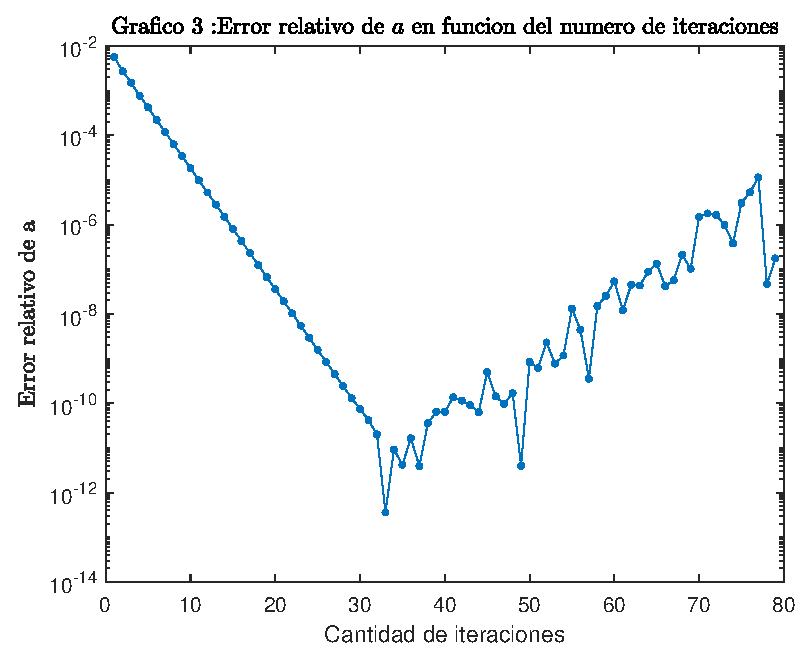
\includegraphics [width=4in]{T1_Murillo_03.eps}
\end{figure}

\begin{par}
	La convergencia parece ser más rápida en el 4c sin embargo, no para todas las iteraciones pues después de treinta y tres el error comienza a oscilar.
\end{par}

\begin{par}
	El gráfico decrece de forma lineal aproximadamente hasta la iteración treinta, después de eso oscila, después de la iteración treinta no presenta monotonía, i.e. el error decrece linealmente hasta 30 y después oscila.
\end{par}

\begin{par}
	5a)
\end{par}

\begin{lstlisting}
load('dataPolin.mat')

size(dataX)
size (dataY)
\end{lstlisting}

\begin{lstlisting}

ans =

    11     1


ans =

    11     1


\end{lstlisting}
    
\begin{par}
	5b)
\end{par}

\begin{lstlisting}
pn = polyfit(dataX, dataY, 10)
\end{lstlisting}

\begin{lstlisting}

pn =

  Columns 1 through 7

   31.2177 -120.1321  -90.8847  245.8358   90.1895 -159.6097  -34.4710

  Columns 8 through 11

   36.0627    3.8656   -1.9053    0.5853


\end{lstlisting}
    
\begin{par}
	La salida pn se interpreta como los coeficientes de un polinomio de grado 10. Este debe ser de grado 10 pues hay 10 + 1 nodos.
\end{par}
\\
\begin{par}
	5c)
\end{par}

\begin{lstlisting}
xx = linspace(-1,1);
yy = polyval(pn, xx);

figure
plot(xx,yy), hold on
plot(dataX,dataY,'.', 'MarkerSize', 15)

%Titulo
title('Gráfico 4 :Polinomio de interpolación')

%Nombrar ejes
ylabel('Polinomio pn')
xlabel('Intervalos')
\end{lstlisting}

\begin{figure}[h!]
\centering
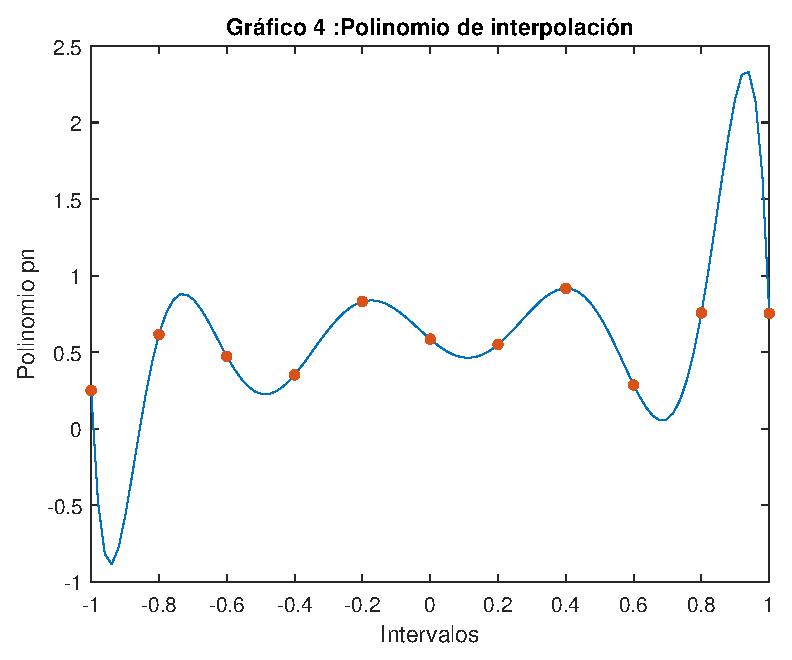
\includegraphics [width=4in]{T1_Murillo_04.eps}
\end{figure}

\begin{par}
	5d)
\end{par}

\begin{lstlisting}
%Creamos dos vectores que contengan los datos de los nodos 1,5,10
nodos_nuevosX = [dataX(1) dataX(5) dataX(10)];
nodos_nuevosY = [dataY(1) dataY(5) dataY(10)];

pn_nuevo = polyfit(nodos_nuevosX, nodos_nuevosY, 2);
yy_1 = polyval(pn_nuevo, xx);

figure
plot(xx,yy_1), hold on
plot(nodos_nuevosX, nodos_nuevosY,'.', 'MarkerSize', 15)

%Titulo
title('Gráfico 5 :Polinomio de interpolación')

%Nombrar ejes
ylabel('Polinomio pn')
xlabel('Intervalos')
\end{lstlisting}

\begin{figure}[h!]
\centering
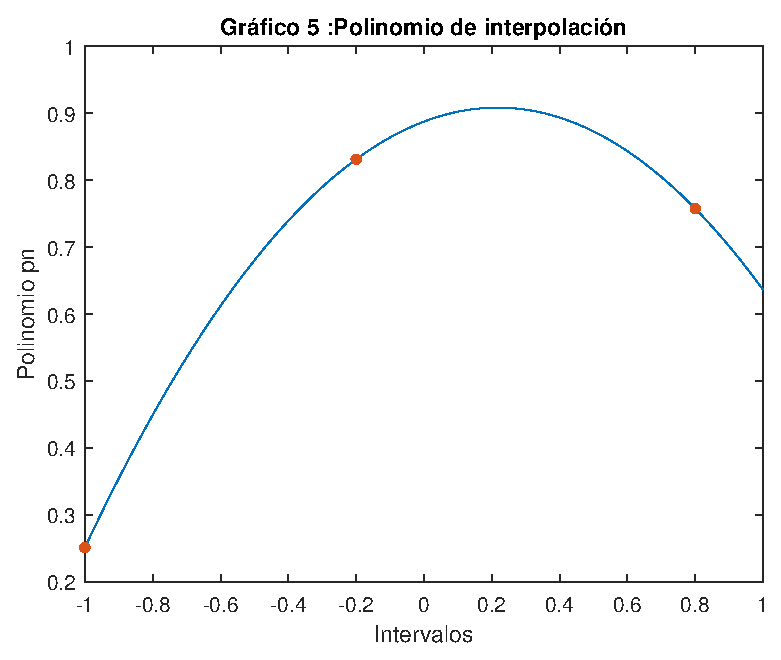
\includegraphics [width=4in]{T1_Murillo_05.eps}
\end{figure}

\begin{par}
	Cuál es mejor? No tiene sentido realizar esta pregunta pues son funciones
realizadas con diferente cantidad de nodos.
\end{par}

\begin{lstlisting}
close all
\end{lstlisting}

\begin{par}
	\textbf{Código de funciones}
\end{par}


\subsection*{Funciones}


\begin{lstlisting}
function c1 = myDivision(c0, b)
    c1 = c0 + c0.*(1 -b.*c0);

    while(abs(c1-c0)>=eps)
        c0 = c1;
        c1 = c0 + c0.*(1 -b.*c0);

    end
end

function [root,seq] = iterSimple(f,x0)
    Tol = eps;
    iterMax = 80;
    k = 1;
    seq = [x0 f(x0)];
    while(Tol && k<iterMax)
        seq = [seq f(seq(end))];
        k = k+1;
    end
    root = seq(end);
end

function [root,seq] = Secante(f,x0,x1)
  Tol = 1e-8;
  iterMax = 100;
  count = 0;
  f0 = f(x0);
  f1 = f(x1);
  if(abs(f0)<Tol)
      root = x0; seq = x0;
  elseif(abs(f1)<Tol)
      root = x1; seq = x1;
  else
      seq = zeros(iterMax,1);
      xNew = x1 - f1*(x1-x0)/(f1-f0);
      fNew = f(xNew);
      seq(count+1) = xNew;
      while(count<iterMax && abs(x1-x0)>Tol)
        count = count + 1;
        x0 = x1;
        x1 = xNew;
        f0 = f1;
        f1 = fNew;
        xNew = x1 - f1*(x1-x0)/(f1-f0);
        fNew = f(xNew);
        seq(count+1) = xNew;
      end
      root = xNew;
      seq = seq(1:count+1);
  end
end
\end{lstlisting}



\end{document}
    
